\documentclass{article}
\usepackage[margin=1in]{geometry}
\usepackage{setspace}
\usepackage{amsmath}
\usepackage{amssymb}
\usepackage{physics}
\usepackage{graphicx}
\usepackage{relsize}

\title{Math 180 Midterm 1}
\author{Jiaping Zeng}
\date{10/30/2020}

\begin{document}
\setstretch{1.5}

\newpage
\begin{itemize}
    \item [Q1] I certify on my honor that I have neither given nor received any help, or used any non-permitted resources, while completing this evaluation.\\
          Signature:
\includegraphics[width=2in]{signature.png}\\
          Date: 10/26/2020
\end{itemize}


\newpage
\begin{itemize}
    \item [Q2] Prove that an Eulerian graph with more than one vertex must have at least 3 vertices with the same degree. (Hint: partition the vertices)\\
          \textbf{Answer}: By contradiction. Let $n=\abs*{V(G)}$ and suppose that at most 2 vertices have the same degree. Then since each vertex in an Eulerian graph has to have an even degree, our possible degrees for each vertex are the even terms from 2 to $n-1$, giving us at most $\frac{n-1}{2}$ possible degrees. Since by our assumption we can have at most 2 vertices per degree, we can only have at most $n-1$ vertices, which contradicts with our assumption of $n=\abs*{V(G)}$. Therefore an Eulerian graph with more than one vertex must have at least 3 vertices with the same degree.
\end{itemize}

\newpage
\begin{itemize}
    \item [Q3] Consider the following sequence \[(4,4,4,4,5,5,6)\]
          \begin{enumerate}
              \item Prove that the sequence above is a valid degree sequence (score).\\
                    \textbf{Answer}: By theorem 4.3.3, we can reduce the sequence as follows:\\
                    $(4,4,4,4,5,5,6)$\\
                    $(3,3,3,3,4,4)$\\
                    $(2,2,2,2,3)$\\
                    $(1,1,1,1)$\\
                    $(0,0,0)$\\
                    Since the last sequence is a graph score, the original must also be a score of some graph.
              \item Prove that a graph with the score above cannot be planar.\\
                    \textbf{Answer}: By theorem 6.3.3, a planar graph with at least 3 vertices must satisfy $\abs*{E}\leq 3\abs*{V}-6$. Using the given sequence, we have $\abs*{V}=7$, so $3\abs*{V}-6=15$. However, $\abs*{E}=\frac{1}{2}\sum_{v\in V}\deg_G(v)=16>15=3\abs*{V}-6$. Therefore the graph cannot be planar.
              \item Draw a graph with the score above.\\
                    \textbf{Answer}:
                    \begin{center}
                        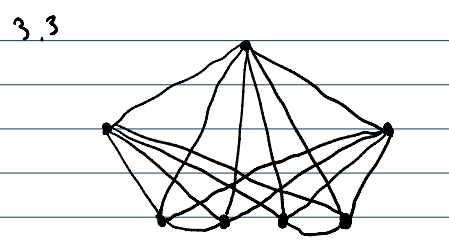
\includegraphics[width=3in]{3-3.png}
                    \end{center}
          \end{enumerate}
\end{itemize}

\newpage
\begin{itemize}
    \item [4.] Consider the following graph $G$ below:
          \begin{center}
              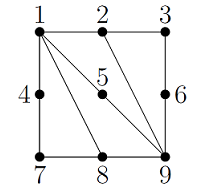
\includegraphics[width=1in]{q4.png}
          \end{center}
          \begin{enumerate}
              \item Does $G$ have an Eulerian cycle?\\
                    \textbf{Answer}: No; since vertices 2 and 8 have odd degrees, by theorem 4.4.1 $G$ cannot be Eulerian.
              \item Determine the connectivity of $G$.\\
                    \textbf{Answer}: $G$ is 2-connected as removing 2 edges from vertices 3,4,5,6 or 7 would disconnect the vertex and therefore disconnect the graph. It is not 1-connected as every vertex is in a cycle.
              \item Is $G$ bipartite?\\
                    \textbf{Answer}: Yes; as follows:
                    \begin{center}
                        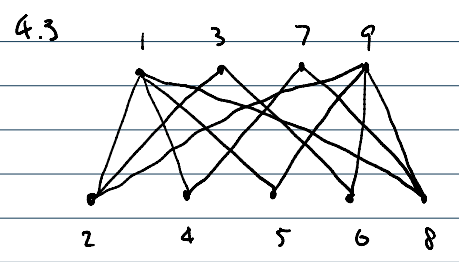
\includegraphics[width=3in]{4-3.png}
                    \end{center}
          \end{enumerate}
\end{itemize}

\newpage
\begin{itemize}
    \item [5.] Let $G=(V,E)$ be a graph whose vertices are the 2-element subsets of $\{1,2,3,4,5\}$. Declare two vertices adjacent if the subsets are disjoint.
          \begin{enumerate}
              \item Prove that each vertex has degree 3.\\
                    \textbf{Answer}: Take an abitrary vertex $(a,b),a\neq b$ from G, $(a,b)$ is adjacent to any tuple from the set $\{1,2,3,4,5\}\setminus\{a,b\}$, which is a set of size 3. Then there are $\binom{3}{2}=3$ choices for 2-element subsets, i.e. $(a,b)$ is adjacent to exactly 3 other vertices. Therefore each vertex has degree 3.
              \item Prove that the shortest cycle in $G$ has length 5.\\
                    \textbf{Answer}: Since a cycle needs to have at least length 3, we will prove the statement by showing that cycles in $G$ cannot be length 3 or 4.\\
                    To contruct a cycle of length 3, we need 3 disjoint 2-element subsets of $\{1,2,3,4,5\}$ since each vertex is connected to the other two in a cycle of length 3. However, it is clearly impossible to construct 3 disjoint 2-element subsets as there are only 5 elements in $\{1,2,3,4,5\}$.\\
                    Now let's try to construct a cycle of length 4. Let $a,b,c,d,e\in\{1,2,3,4,5\}$ be distinct. Then let arbitrary $(a,b)$ be the starting vertex and $(c,d)$ be the second vertex. The third vertex then is selected from $\{a,b,e\}$; since we cannot have duplicate vertex $(a,b)$, we can only have $(a,e)$ or $(b,e)$. Then the fourth vertex is selected from $\{b,c,d\}$ or $\{a,c,d\}$; since we cannot select duplicate vertex $(c,d)$, either $a$ or $b$ must be a part of the fourth vertex. But this means that the fourth vertex is not disjoint to $(a,b)$, and therefore such cycle of length 4 does not exist.
              \item Prove that $G$ is not planar.\\
                    \textbf{Answer}:
                    \begin{center}
                        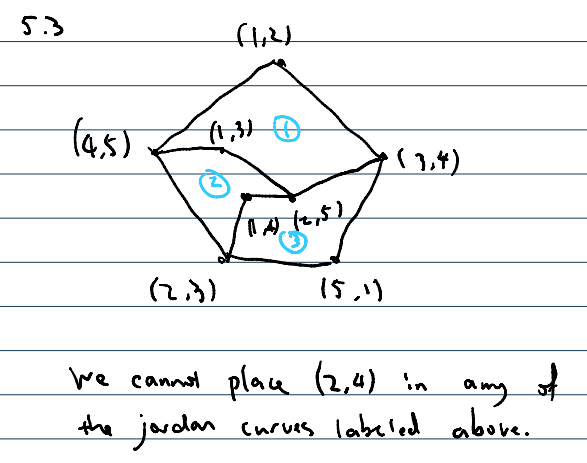
\includegraphics[width=3in]{5-3.png}
                    \end{center}
                    Proof by contraction. Since the vertices $(1,2),(3,4),(5,1),(2,3),(4,5)$ form a cycle, the arcs $\alpha[(1,2),(3,4)]$, $\alpha[(3,4),(5,1)]$, $\alpha[(5,1),(2,3)]$ and $\alpha[(2,3),(4,5)]$ form a Jordan curve $k$. Now take the vertices pair $((1,3),(2,4))$; since they are disjoint subsets, they must be connected. Therefore they must be either both inside $k$ or both outside $k$ or $\alpha[(1,3),(2,4)]$ would intersect $k$. Similarly, the same must apply for the pairs $((1,4),(2,5))$ and $((1,3),(2,5))$.\\
                    Suppose $(1,3)$ lies inside $k$, then so does $(2,5)$; since $(2,5)$ is now inside $k$, then so is $(1,4)$. Then $k$ is divided into three Jordan curves by these three vertices and their edges as shown in the diagram.\\
                    Now consider the vertex $(2,4)$, which must be inside $k$ as shown previously. However, on the one hand, if we place $(2,4)$ inside either Jordan curves 1 or 2, as labeled in the diagram, the edge $((2,4),(5,1))$ would intersect at least one Jordan curve. On the other hand, if we place $(2,4)$ inside Jordan curve 3, the edge $((2,4),(1,3))$ would intersect at least one Jordan curve.\\
                    If $(1,3)$ and $(2,4)$ lie both outside $k$, we can proceed analogously. Therefore $G$ is not planar by Jordan curve theorem.
                    
          \end{enumerate}
\end{itemize}

\newpage
\begin{itemize}
    \item [6.] Let $G=(V,E)$ be a graph and let $e\in E$ be an edge.
          \begin{enumerate}
              \item Express $\abs*{E(G/e)}$ in terms of $E(G)$ and $T_e(G)$, the number of triangles in $G$ containing $e$ as an edge.\\
                    \textbf{Answer}: Since $e$ is not in $G/e$, we lose it when contracting $e$. In addition, every triangle that contains $e$ becomes a single edge, losing an additional edge per triangle. Therefore we have $\abs*{E(G/e)}=\abs*{E(G)}-T_e(G)-1$.
              \item Let $T(G)$ be the number of triangles in the graph $G$. How are $T(G)$, $T(G-e)$ and $T_e(G)$ related?\\
                    \textbf{Answer}: Since $G-e$ is formed by removing $e$ from $G$, $T(G)$ differs from $T(G-e)$ by $T_e(G)$, i.e. $T(G)=T(G-e)+T_e(G)$.
              \item Let \[P_G(x)=x^n-a_{n-1}x^{n-1}+a_{n-2}x^{n-2}-\ldots\] be the chromatic polynomial of $G$. Recall that $a_{n-1}=\abs*{E(G)}$. Prove (by induction on the number of edges) that \[a_{n-2}=\binom{\abs*{E(G)}}{2}-T(G)\]
                    \textbf{Answer}: Proof by induction as follows.\\
                    Base case:\\$\abs*{E(G)}=2$ (no triangle); then $P_G(x)=x(x-1)^2=x^3-2x^2+x$. So $a_{n-2}=1=\binom{2}{2}-0$.\\
                    $\abs*{E(G)}=3$ (one triangle); then $P_G(x)=x(x-1)(x-2)=x^3-3x^2+2x$. So $a_{n-2}=2=\binom{3}{2}-1$.\\
                        Inductive step:\\
                        Suppose $a_{n-2}=\binom{m-1}{2}-T(G)$ holds for $m-1$ edges. We want to show that it will also hold for $m$ edges. By the Fundamental Reduction Theorem, for an edge $e$, we have $P_G(x)=P(G-e,x)-P(G/e,x)$. By inductive hypothesis, the coefficient for the $x^{n-2}$ term in $P(G-e,x)$ is $\binom{m-1}{2}-T(G-e)$. In addition since $P(G/e,x)$ is a degree $n-1$ polynomial (by homework 3 P2), its coefficient for the $x^{n-2}$ term is $-\abs*{E(G/e)}$, which is equivalent to $\abs*{E(G)}-T_e(G)-1$ by part (a). So we have $a_{n-2}=\binom{m-1}{2}-T(G-e)+\abs*{E(G)}-T_e(G)-1=[\binom{m-1}{2}+m-1]-[T(G-e)-T_e(G)]$.\\
                        We can tackle the two parts of the above expression separately as follows: the left term simplifies to $\binom{m-1}{2}+m-1=\frac{(m-1)!}{2!(m-1-2)!}+\frac{2(m-1)}{2}=\frac{(m-1)(m-2)+2(m-1)}{2}=\frac{(m-1)[(m-2)+2]}{2}=\frac{m(m-1)}{2}=\binom{m}{2}$. The right term simplies to $T(G-e)-T_e(G)=T(G)$ by part (b). Then by substitution we have $a_{n-2}=[\binom{m-1}{2}+m-1]-[T(G-e)-T_e(G)]=\binom{\abs*{E(G)}}{2}-T(G)$.\\
                        Therefore $a_{n-2}=\binom{\abs*{E(G)}}{2}-T(G)$ by mathematical induction.
          \end{enumerate}
\end{itemize}
\end{document}